%!TEX root = thesis.tex
\chapter{Cache Oriented Obfuscation}

In this chapter of the thesis, we proposed a method to design a reliable and efficient obfuscation technique for tightly coupled multi-processing systems by exploiting the feature of cache oriented programming. Besides, we emphasized a number of points to characterize proper attack vector. After we had elaborated our obfuscation methods and its primitives, we discussed what it is and what it is not on pitfalls and fallacies section. Finally, on the implementation section, we drew a picture of possibilities for practical applications. However, this chapter and this thesis do not concern specific and deeper studies on obfuscation and memory protection(TLB, MMU, MPU). They are correlated with our thesis, but it is in the upper layer which is like TCP and IP layers of the network. On the whole and in the brief, this chapter gives an isolated workspace for obfuscation techniques.

As we mentioned previous chapters, malware detection tools needs sensors to analysis running code. Regular sensors observes real-time systems with monitoring shared memory, it means a lot for operating systems, because OS, computer architecture and computer conventions assume everything on the memory and ultimate and consistent. With this assumption, dumping memory and analyzing snapshots are practically an efficient and convenient way of malware monitoring and detecting. There are actually a number of sensor type for real time memory observation: external monitors, internal monitors, and exotically virtual monitoring. External monitors in contrast with internal monitors are the systems which is comprised with external hardware devices and its software component. They could be implemented on external PCI or GPU devices, FPGA co-processor or on-board chip\cite{Christos2013}. They are efficient because they are pre-installed, omnipresent systems which does not require OS and other middleware platform which constrains their limits. Also, They are efficient because they are the hardwares which can be designed with the purpose. However, they are expensive to implement comparing to internal monitors. Internal monitors are using regular devices on the computer architecture such as CPU, and they are working under the operating system's kernel, which could be easy to deceive \cite{Adnan2011}, \cite{rutkowska2006rootkits}. Our methods is actually not depending on the monitoring type, since it is related to where they are monitoring.
    \begin{figure}[h!]
        \centering
        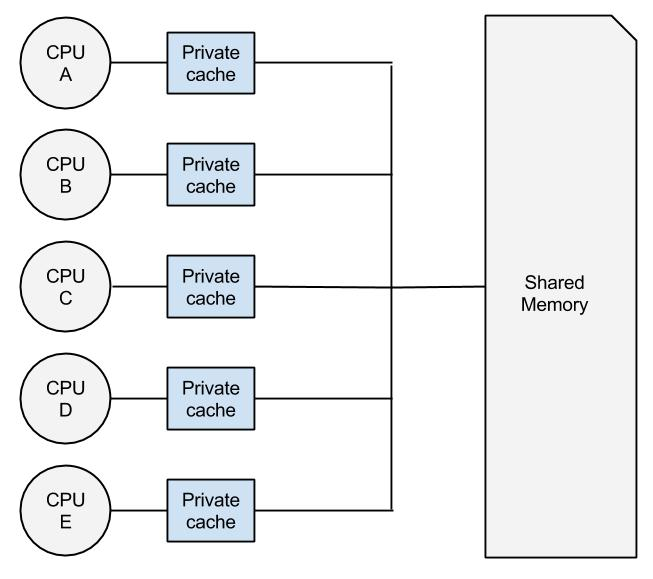
\includegraphics[width=1\textwidth]{img/Tightly Coupled Multi-Processing Systems.jpg}
        \caption{An Example of Tightly Coupled Multi-Processing Systems}
        \label{fig:tightlycoupled}
    \end{figure}
Tightly coupled multi-processing systems have many processors with their own caches and one shared memory\cite{Jim2007}. Cache memories are not developed with the same purpose with memories, but they are developed for performance reason which we discussed in background studies. If we exploit them and design our program properly, cache memories could behave as another layer of memories, and on the monitoring side, even if it scan perfectly memory(s) and detect malicious codes, cache memories are still out of the box.

The required systems for our technique in this chapter is tightly coupled multi-processing systems without cache coherence interconnector. Also, we need simple Harvard computer architecture instead of Von Neumann. Incoherent systems are surprisingly popular because of the implementation errors i.e. Samsung's mainstream CPU Exynos 5410 which sold millions, and also due to costs. Many hardware designers also believe programming with shared memory is not appropriate way and platforms such as Android already using message based communication on multi-threaded application, and  they implement clustered processors which limits programs instead of implementing expensive coherency interconnector. Yet, they have not considered security approaches.

	

	\section{Exploiting Tightly Coupled Multi-Processing Systems}
	
	    \begin{figure}[h!]
	        \centering
	        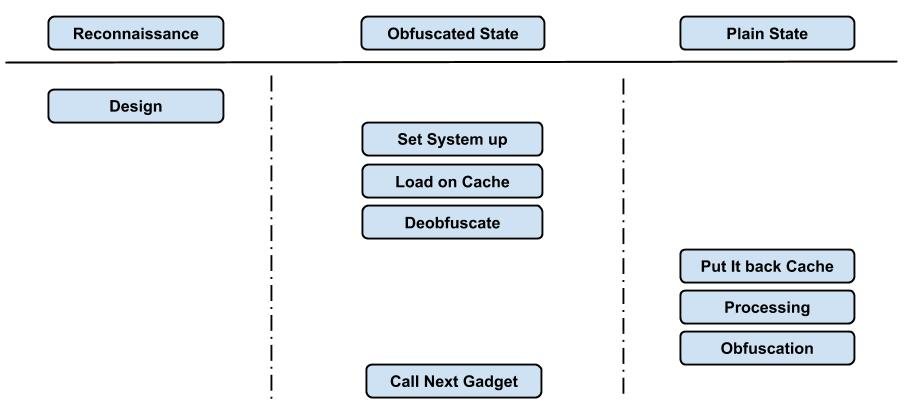
\includegraphics[width=1\textwidth]{img/attack_vector.jpg}
	        \caption{Attack vector flow chart}
	        \label{fig:atackvector}
	    \end{figure}
	    In this section, we will formulate our attack vector one by one, and we will show implementation and theoretical obstacles. Essence of the thesis is exploiting caches to hide values from upper layer memories but also it concern some subtle studies to run a comprehensive code from beginning to end. In figure \ref{fig:atackvector}, our attack vector flow chart showed. There is no doubt that most important part of our attack is designing and reconnaissance part, because after we produce cache oriented malware, it is a kind of system depended malware and can't work on the every systems, but can be useful as targeted attacks (e.g Stuxnet). Targeted attacks could be really efficient because of the facts that, all anti malware tools aims massive market, and if malware aims sneakily small portion of the market, they could be successful forever. Setting system up and loading memory second step of the attack vector and first step of attack loop. In this section, we will show cache tricks and explain why it is efficient. In the last chapter we will emphases obfuscation and deobfuscation methods briefly, and we will discuss some control flow issues. As you can see, when code or data is deobfuscated, it is on the cache memory. When we call the next independent part of the code, it must definitely be obfuscated back, because we do not want to evict cache blocks to memory plain. 
	    \subsection{Reconnaissance and Design}

	    Design and reconnaissance is the most crucial part of our attack approach, because the size of the cache memory is the basic dependence. If you try to fill more data than its actual size to cache memory, it evicts a number of cache blocks depending on the replacement policy. It is what really we do not want, if the evicted block are not obfuscated. Our first design approach to prevent leakage of plain data upper layer of the cache memory. As we have seen in background chapter, cache are a kind of memories but it also comprise with logical circuit to replace its block autonomously, because they are incomparably small and depending on the main memory to store and load informations. If we claimed they are invisible layer between memory and processors, it would not be totally wrong, and also many programmers today do not concern about their performance feature when they design their program's loops. On the other side, if you consider cache properties while designing your programs, It is hard to determine the base system. For example if we have 32 byte cache block, we could consider when we load an address it will load 32 byte into the cache and in the most frequently working look could progress on this values e.g. arrays are continues bytes and they are generally loading all together. However, cache sizes are extremely various today on the market and if you design a cache oriented program for 32 byte cache block it will not work properly on the cache which has 20 cache block size. Beside that fact, cache size is also important constraint and worst, they have more various then cache block size on the market.

	    Therefore, we propose to generate a specific piece of code to fit for each cache corresponding to cache size, cache characteristic and also target system  arch and security level. Target system architecture may imply cache architecture, and we could design more complex and more flex gadget with multi layer cache arch. if many processors can reach a cache and share values, we could easily broke control flow graph\cite{ramilli2011multiprocess}, and also on the higher level caches we should use more memory space comparing with lower layer, but if and only if there is no malware sensor which is monitoring memory, we should use upper layer of memory. When we are using a CPU, it is quite certain that it is the only one who is accessing corresponding cache. In figure \ref{fig:gadgetsections}, illustration of a gadget is showed. It has two sections which are stub and body. This body section is loaded with actual gadget code and tail section. Tail section is responsible with stitching gadget properly. So every gadgets knows before they started to run, which gadget they are followed by. It is a bit problematic and tricky, see Pitfalls and Fallacies section for details.

	    When we determine the gadgets size, we should consider the cache properties, such as replacement policy, block size, set associativity, line size and total size of cache. The size of gadget must not be more than the total size of cache, and also must be designed with no eviction before obfuscation principles. Hence, we must know who will be evicted next always. On random eviction model, we should not consider eviction during processing of gadget. During running a gadget code, also we must be sure there is memory load or store operation to memory except gadget memory space. Also all gadget must be adjusted to settle in memory continuously in order to utilize spacial locality.

	    \begin{figure}[h!]
	        \centering
	        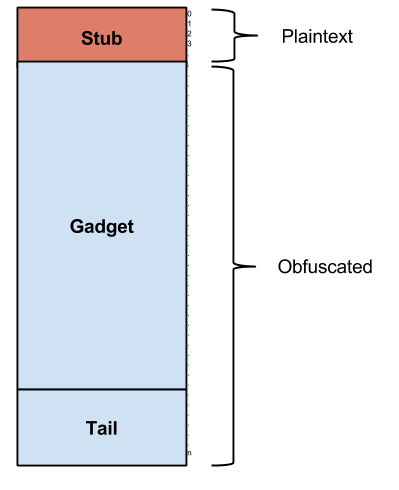
\includegraphics[width=0.5\textwidth]{img/Code_illustration.png}
	        \caption{Gadget Sections}
	        \label{fig:gadgetsections}
	    \end{figure}

 	    \subsection{Setting System up and Loading Cache Memory} 

 	    	The second step of our attack is to settle on target system. It was the first step on target machine. In order to load all gadgets into the memory, we should use a kind of middle-ware to carry them. In conventional computer architecture and operating system internal, there is not many way to do this. Since volatility of main memory, code must be keep under a kind of I/O devices. This devices are generally connected to DMA devices which provide direct access of I/O devices to main memory. It is a short cut to avoid flooding CPU for each request\cite{mmap2011}. Reading this devices from scratch is not simple task, because CPU instruction and memory maps allow you to read sectors or blocks on the disk, and this could be meaningless without proper structure e.g. FAT, LDM, Raid. Instead, we recommend to use OS or boot-loader features to read files. In listing \ref{code:bootloader}, we showed an example for loading a gadget from disk 0 to memory and set instruction pointer to first memory block of gadget on U-BOOT\footnote{U-Boot is the one of the most common ARM boot-loader by Denx Engineering}. It is a method as if a rootkit could use, because it load itself just before OS is loaded. In this case, Keep in mind that you should initialize OS kernel on the other processor later. On the other hand, On OS implementation, you gadget should be covered with executable structures such as ELF or PE. The most important point here is when you define your structures you should define your gadget part as executable, writeable and readable; therefore, you can deobfuscate executable code.

 	    	\begin{lstlisting}[caption=The code example for loading a gadget from disk to memory and run it on U-Boot, label=code:bootloader]
mmc dev 0; 	#Device Number
fatload mmc 0:1 ${addr_r} gadget_file;
go ${addr_r};
 	    	\end{lstlisting}

 	    	One of the other attentive point is choosing appropriate address for loading first byte of gadget. It is really crucial, for all gadgets are designed to size of cache as we mention in previous section. If you start to fetch a gadget to the wrong block in memory, then the gadget overflows cache size, although gadget size is right. As we mention in background studies chapter, cache memories have some internal organization. Therefore, before gadgets are fetching from disk to memory, the first address of each gadgets must be predetermined as fit for the first block of any cache line. In other words, the first bit of the gadget must be loaded in a memory address which is first block of any cache line. If it starts in the middle and passes $x$ block, it overflow x block at the end and when it is requested by CPU, it will evict a set in first cache line depending on replacement policy. To calculate first block addresses, we can use formula below.

 	    	\begin{equation}
 	    		S = \{address | 0\equiv address \bmod{cache line size}\} \quad
 	    		\forall x \in S := first cache block
 	    	\end{equation} 

			\begin{lstlisting}[caption=The code example for loading a section of memory to cache, label=code:memtocache]
	mov R2, 0x012345 #address
	mov R3, 0x013456 #end of gadget
fetch: 	
	mov R1, [R2] #Load address from memory
	addi R2, 4 # add size of word to address
	cmp R2,R3 # compare R2 and R3
	jl fetch
			\end{lstlisting}

			The code which is showed above in listing \ref{code:memtocache} shows the primitive method for fetching memory section into cache memory. Beside of this, you can enhance this code with adding steps between memory location it fetched, because you do not need to fetch each word as showed above. Instead, you can skip $cachelinesize - wordsize$ byte. The cache controller autonomously fetch the following blocks to exploit spacial locality as we mention in previous chapter. Although every further attempt to fetch word will be loaded from cache memory and it is faster then memory access, stepping approach is always better. On this X86 similar assembly code example, on the first two line, it move the first and last address of the gadget into R2 register. Then, it starts loop and fetches incrementally location in the memory, and when it reach to the ending address it jumps out of loop. 
	    \subsection{Obfuscating, Running and Deobfuscating Gadget}
			After we load the gadget into the cache, it is time to deobfuscate it to run it. There are many buzz term for obfuscation methods and techniques such as polymorphism, metamorphism, omnimorphism and homomorphism\cite{nachenberg1996understanding}\cite{li2011mechanisms}\cite{marpaung2012survey}\cite{balakrishnan2005code}. However, in this paper, we don't mention the details of these techniques, but instead we will emphases highlights. The most obvious key is that it is not disk to memory obfuscation, it has quite little place to use in cache, so we can not use complicated obfuscation algorithms. 

			Most known methods we have known so far are $XOR$ and $NOT$ operations. $NOT$ operation does not require key to deobfuscate it, though $XOR$ need. Key could be useful against advance malware detection methods because it is quite common that anti malware software are checking signatures and also their $NOT$ state. Even though $XOR$ needs key and can change it after every obfuscation deobfuscation operation, there are techniques to deobfuscate $XOR$ patters simply since key is stored plainly somewhere in stub part, and it is also reason why we call it obfuscation instead of encryption. Sequential $XOR$ keys are also well known attack against generic $XOR$ decryption which is influenced by enigma and solved like enigma i.e. entropy analysis of assembly instruction. Custom obfuscation algorithms are also another method to obfuscate, but the vital point to design obfuscation algorithms, well known and commonly used algorithms should be preferred because the deobfuscation algorithm and key are in stub part. It is pretty easy to detect, identify and signature unique algorithms, so with manual analysis, signature could be obtain and used to detect our stub part. To solve this, well known encryption algorithms such as DES or a specific part of them can be used.
	    \begin{lstlisting}[caption=The code example of obfuscation and deobfuscation routine, label=code:obfuscation, numbers=left, numberstyle=\tiny]
	mov R2, 0x012344 	#start address of body
	mov R3, 0x013456 	#end of gadget
	mov R4,0
obfuscate: 
	mov R1, [R2] 		#Load address from cache
	xor R1, 12345 		#key
	mov [R2], R1
	addi R2, 4 		#add size of word to address
	cmp R2,R3 		#compare R2 and R3
	jne obfuscate
	cmp R4,0
	jne R4 			#jump next gadget
start_addr_body:
	...
	...
	...
	...
tail_addr:
	mov R4, 0x234568 	#next gadget
	mov R2, 0x012344
	jmp obfuscate
end_addr:
		\end{lstlisting}

			On the figure \ref{fig:gadgetsections}, a typical gadget compartments are showed. It has stub and body parts. Stub part consists deobfuscation algorithm and key(s). It must be usual code which is using frequently, so it can not be identical. Body part consist two subsection which are called gadget body and tail. Gadget body is actual code which is a part of malware. Tail part is a part for maintaining obfuscation process as like as stub part. In tail part, it can regenerate stub part in order to obtain uniqueness on every attempt, but it is baroque job to fit in cache size. Instead, we can change key for each attempt. After we regenerate stub part, then we should obfuscate body part. 

			On the listing \ref{code:obfuscation}, a primitive code sample showed for obfuscation and deobfuscation routine. The compartments of the gadget can be seen roughly on the code example. From beginning of the chapter to $start_addr_body$, it is $stub$ part, and rest of it is body. Tail of the body part start from $tail_addr$ to end of code. As you can see in this example, tail code is not obfuscated state. The area with ellipsis belongs to gadget body which is actual malware. The first three line is to initiate loop. As we fetched the gadget to the cache on previous section, we started to work on cache in this section. from line 5 to 8, it is actual obfuscation and deobfuscation part. We used here static key but it is easy to use dynamic key with a register. First jump instruction on line 10 is checking for loop variables, and second jump on line 12 is checking for whether it is obfuscation or deobfuscation state. In this example, we used common code to obfuscate and deobfuscate. It is quite efficient with symmetric obfuscation techniques. After it complete deobfuscation of whole body part, it naturally goes in body part, then at the end, it jumps to obfuscation section after it sets $R4$ register with start address of next gadget's $stub$. At the end of the gadget, it runs instruction on line 12 which jumps new gadget, therefore; it evicts cachelines and fetches its own gadget and do all these routines. We consider that all these gadgets works as a loop of gadgets, so it does not need to have exception or interrupt between gadgets transactions.


		    \begin{figure}[h!]
	        \centering
	        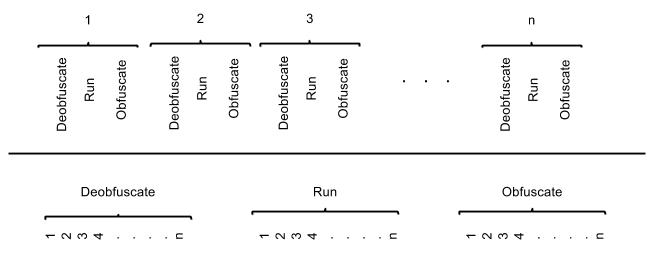
\includegraphics[width=1\textwidth]{img/control_flow.jpg}
	        \caption{Control Flow Illustration A) Stepped Control Flow B) All at Once Control Flow}
	        \label{fig:controlflow}
	    \end{figure}
	        We will also propose two type of control flow method for obfuscation, running and deobfuscation routine. In figure \ref{fig:controlflow}, these two approach are illustrated which are on the upside "Stepped Control Flow" and on the downside "All at Once Control Flow". Stepped control flow is running instruction one by one in contrast to all at once. Thus even if it leaks some information in the cache memory, it is just an instruction. However, it is barque to implement this control flow due to many reason. It must be perfectly designed before it run, because there must be register convention between stub and gadget and they should not use same registers in the same time. In addition to this should put a $nop$ or junk instruction in a loop and should change the memory of the concerned instruction with new one. In listing \ref{code:control_flow}, the code try to express what it means. The instruction on the memory location 120 is actually junk instruction which is there to be replaced with deobfuscated code, and the instruction on the memory location 116 is to move plain instruction to the junk's place. However, it is not that easy as showed on code, because of the fact that branches. We should consider branches and fetch them in the loop before they are called and it could be made with an interpreter similar code. It is not utopia, but still hard to implement. It is beneficial to emphases one more time that the register in used by obfuscation algorithm must not be used with gadget or stored in a conventional places in case of stepped algorithm usage. This kind of routines are also really common in stack based assembly programming (e.g. calling convention). Instead of stepped control flow approach, all at once approach is easier, faster but less obfuscated. The code in listing \ref{code:obfuscation} is one of example of all at once method. 
	    \begin{lstlisting}[caption=The code example of stepped control flow approach, label=code:control_flow]
100		mov R2, 0x012344 	#start address of body
104		mov R3, 0x013456 	#end of gadget
	loop: 
108		mov R1, [R2] 		#Load address from cache
112		xor R1, 12345 		#key
116		mov [120], R1 		#move ins to junk line
120		nop			#junk line
124		addi R2, 4 		#add size of word to address
128		cmp R2,R3 		#compare R2 and R3
132		jne obfuscate
		\end{lstlisting}


\section{Pitfalls, Limitations and Fallacies}

		The things we mention so far was explained for actually a simple test system which does not have many features of real systems. That makes it simpler and applicable. However, It is not that simple, when implementing on real systems. The systems today we use even in our daily PC are chaotic and baroque. They have many units to make them feasible for our daily usage. In this chapter, we ignored some issues with memory management unit and memory protection units, cache coherency interconnectors, Harvard Architecture, write through cache policy, out of order processors, multi-threading and context switching, and designed our attack for primitive and theoretical computer system, and it could be quite difficult and knotty to implement it on a real system. 

		One of the most important issues which we ignore is definitely interconnectors which provide cache coherency. With increasing of multi processor system usage, it is getting common to implement an interconnector between processors to provide cache coherency. It converts caches to devices which can communicate with each other. All cache memories are assumed coherent, so if a malware work on a CPU and its cache can't conceal its content from another CPU. However, in next chapters we will propose an attack to exploit coherency latency. In any case, it certainly constrains our attack abilities.

		Secondly, on Harvard architecture, There are two different caches which are separate for instruction and data. It breaks our approach throughout. We can work on upper layer cache, e.g L2, L3, but then they generally share the cache with several CPU. We will also propose a novel method to bypass this issue as well.

		Write through caches aren't also perfectly suitable for our attack, but the stepped approach could solve this issue. As it does not need to deobfuscate all code at once, It could reduce the possibility of obtaining signature with leaking a word of memory per time. One word which is about 32 bit size is mostly not adequate to identify a malware. On $stepped$ method, one of the most important obstacle we can encounter is out-of-order and pipelined processors. In stepped approach, all the instructions are nested, and before it write new instruction to the junk instruction place, it might start to decode it or worse might have been already run. Memory barriers and junk delay instructions could be used against this.

		It is a bit tricky to design gadgets, and it constrains functional programming because it is really usual for functions to be independent from the rest of the part, it makes them a suitable candidate to be gadgets. In contrast with functions, gadgets cannot be called again and again. Therefore, we must write another gadget for each use. However, if we convert them to functions with inputs and outputs, it could be an efficient way of designing feasible programs. In addition to functional input and output, they should get the address of gadget which they will stitch with. In order to protect eviction on cache memory, we can use some architectures cache lock. Cache locks can prevent a cache line to evict, in case of fetching its identical pair from memory. If a CPU fetch a memory location, and its corresponding cache line is locked, then the CPU fetches it directly from the memory.